\documentclass[t]{beamer}

%% ----------------------------------------------------- PACKAGES ----------------------------------------------------- %%
\usepackage{coolPrez}

%% ---------------------------------------------------- DOCUMENT ---------------------------------------------------- %%

\begin{document}

%% TITLE PAGE
\title[Learning from noisy demonstrations : a exploration/exploitation tradeoff]{Learning from noisy demonstrations : a exploration/exploitation tradeoff}
\author[Test]{Louis Faury}
\institute[Semester Project at LASA]{Semester Project at LASA}
\titlegraphic{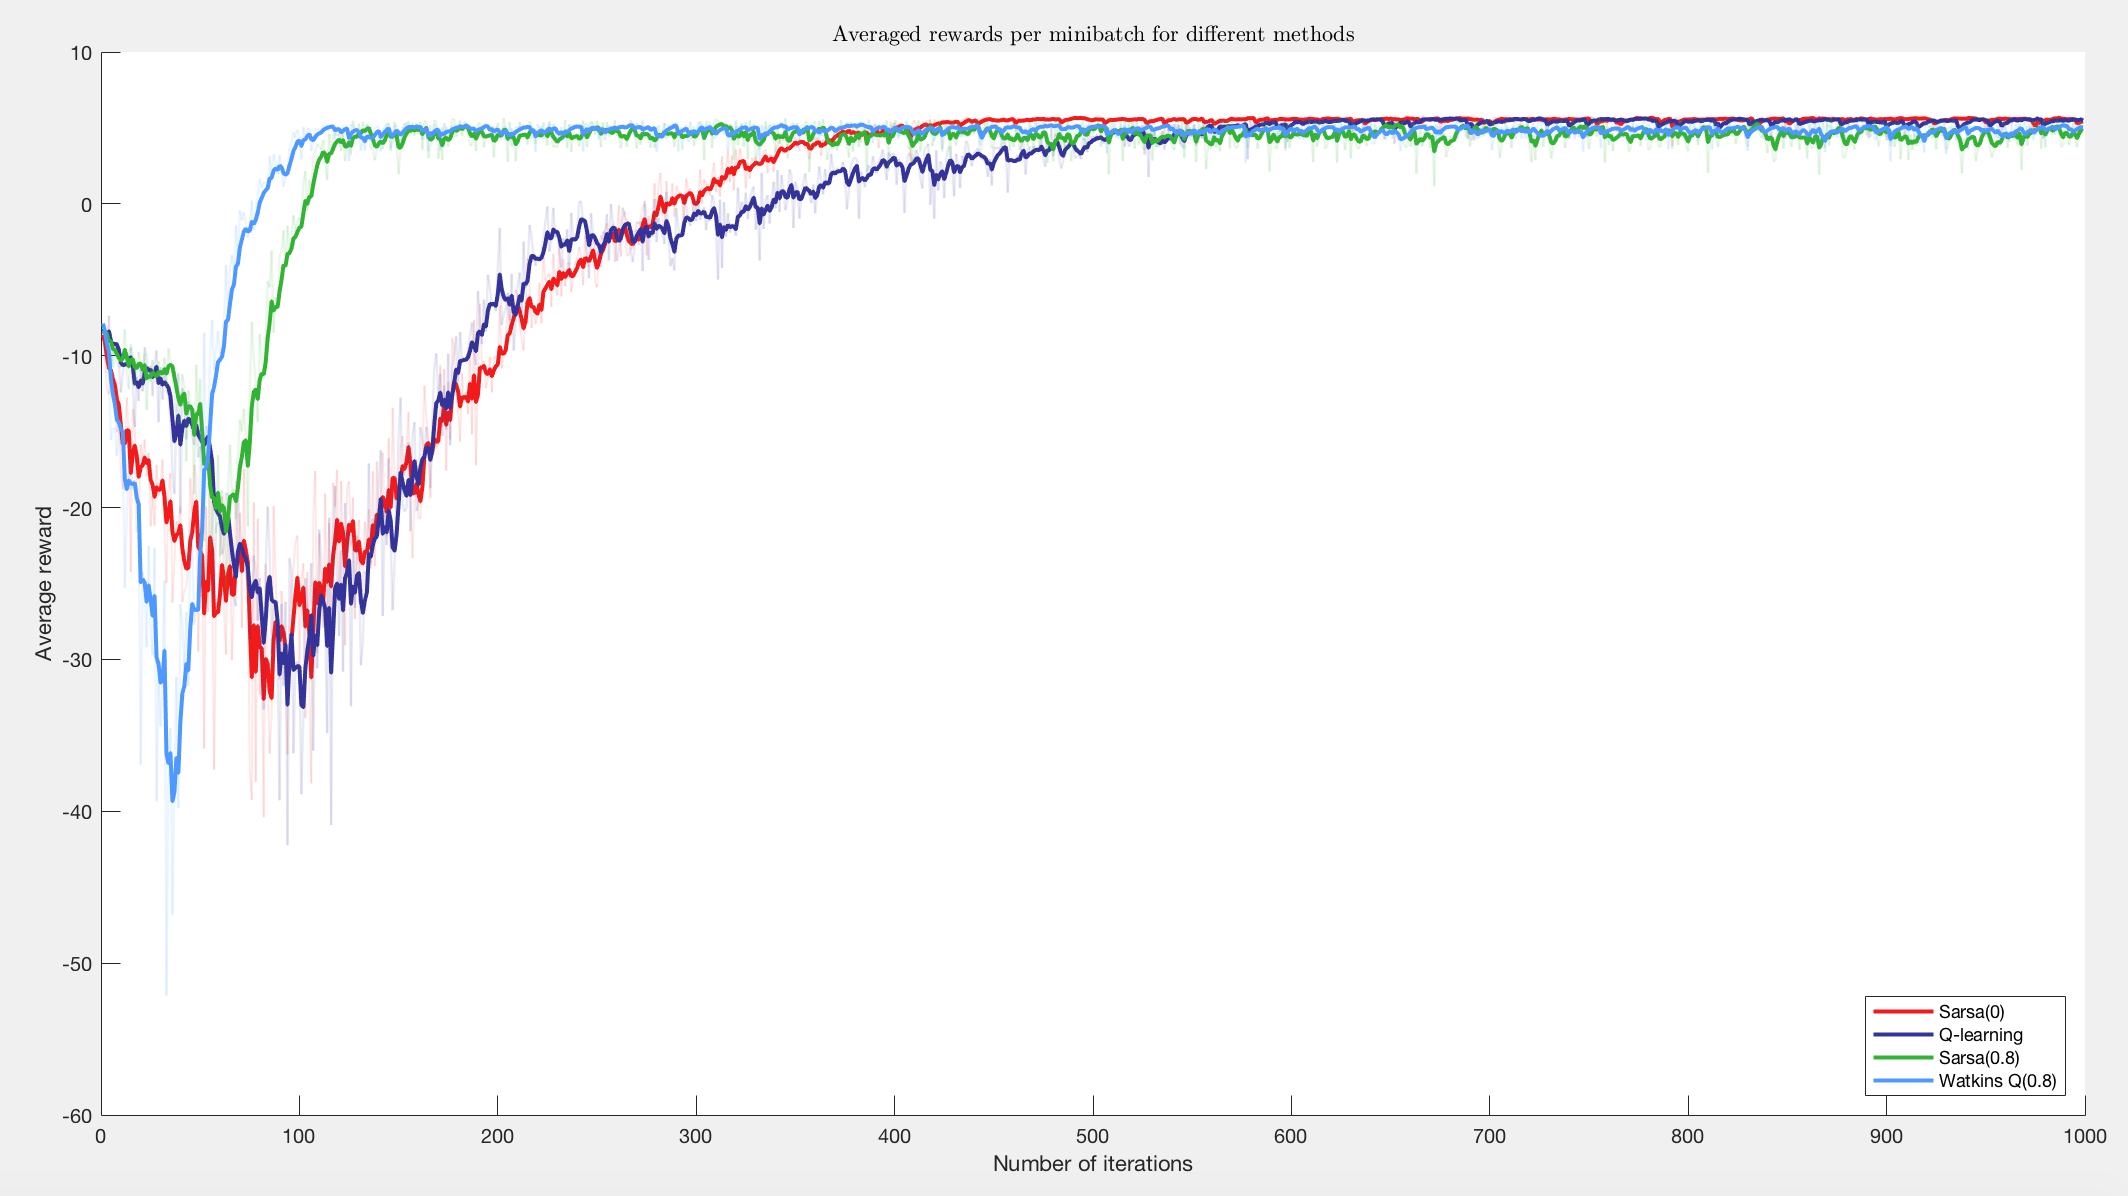
\includegraphics[width=0.8\linewidth]{titlepage_pic}}

\titlepage

%1
\begin{frame}[t]
	\vspace{-3ex}
	\frametitle{Plan}
  	\tableofcontents
\end{frame}

\section{Motivations}
{
	\frame[t]
	{
	
	}
}

\section{Background}
{
	\subsection{Learning from Demonstration}
	{
		\frame[t]
		{
	
		}
	}
	\subsection{Reinforcement learning}
	{
		\frame[t]
		{
	
		}
	}
}

\section{Approach}
{
	\subsection{A sandbox state space}
	{
		\frame[t]
		{
	
		}
	}
	\subsection{RL results}
	{
		\frame[t]
		{
	
		}
	}
	\subsection{Compliance based update rule}
	{
		\frame[t]
		{
	
		}
	}
	\subsection{Results}
	{
		\frame[t]
		{
	
		}
	}
}


%Bibliography
%\bibliography{bib.bib}

\end{document}